\documentclass[a4paper,12pt,fleqn]{book}

% ---------------------------------------------------------------------------
%				Packages
% ---------------------------------------------------------------------------

% texdoc <nom_package> pour avoir des infos
\usepackage{etex}

\usepackage[utf8]{inputenc}						% Encodage français
\usepackage[frenchb]{babel}						% Mise en forme française
\usepackage[T1]{fontenc}						% Encodage caractères français

\usepackage{fourier}							% Différents symboles et polices
\usepackage[scaled=0.875]{helvet}				% Font générale
\usepackage{courier}							% Font télétype
\renewcommand{\ttdefault}{lmtt}					% Font télétype
\usepackage{frcursive}							% Ecriture manuscrite type écolier
\usepackage{calligra}							% Ecriture manuscrite classieuse
\usepackage{verbatim}							% Commentaires

\usepackage{amsfonts,amsmath,amssymb}			% Symboles maths
\usepackage{bm}									% Symboles maths en gras \bm{}
\usepackage{amstext}							% Texte en mode math de taille adaptée
\usepackage{amsopn}								% \DeclareMathOperator
\usepackage{mathrsfs}							% Symboles maths
\usepackage{mathtools}							% Symboles maths
\usepackage{theorem}							% Mise en forme des théorèmes

\usepackage{textcomp}							% Symboles
\usepackage{pifont}								% Symboles "ding"
\usepackage{wasysym}							% Symboles (smiley et logos)
\usepackage{epsdice}							% Symboles (faces d'un dé)
\usepackage[normalem]{ulem}						% Fioritures de texte (barré, etc...)
\usepackage{cancel}								% Barrer du texte (simplifier termes)
\usepackage{fancybox}							% Boîtes

\usepackage{tabularx}							% Tableaux évolués
\usepackage{diagbox}							% Cases en diagonale
%~ \usepackage{tabls}							% Espaces dans les tableaux (conflit avec bclogo)
\usepackage{multirow}							% Fusionner les lignes d'un tableau
\usepackage{enumerate}							% Enumérations personnalisées
\usepackage{multicol}							% Environnement multicolonnes
\usepackage{fancyhdr}							% En-têtes et pieds de page
%~ \usepackage[np]{numprint}					% Mise en forme des nombres

\usepackage[usenames, dvipsnames]{xcolor}		% Couleurs
\usepackage{graphicx}							% Insérer des images
\usepackage{pgf, tikz, tkz-tab, tkz-fct}		% Graphiques avec Tikz
\usetikzlibrary{arrows}
\usetikzlibrary{snakes}
\usepackage{alterqcm}							% QCM
\usepackage{circuitikz}							% Circuit éléctriques
\usepackage[tikz]{bclogo}						% Boites à logo

\usepackage{titlesec}							% Mise en forme des titres de sections
\usepackage{lastpage}							% Dernière page : \pageref{LastPage}

\usepackage{ifthen}								% Programmation conditions
\usepackage{multido}							% Boucles
\usepackage{calc}								% Calculs

% ---------------------------------------------------------------------------
%				Macros simples (caractères)
% ---------------------------------------------------------------------------

\newcommand{\euro}{\eurologo{}}
\newcommand{\R}{\ensuremath{\mathbb{R}}}
\newcommand{\N}{\ensuremath{\mathbb{N}}}
\newcommand{\D}{\ensuremath{\mathbb{D}}}
\newcommand{\Z}{\ensuremath{\mathbb{Z}}}
\newcommand{\Q}{\ensuremath{\mathbb{Q}}}
\newcommand{\C}{\ensuremath{\mathbb{C}}}
\newcommand{\e}{\text{e}}
\renewcommand{\i}{\text{i}}
\newcommand{\s}{\ensuremath{\mathcal{S}}}
\newcommand{\sol}[1]{\mathcal{S}=\left\lbrace #1 \right\rbrace}
\newcommand{\ou}{\mbox{ ou }}
\newcommand{\et}{\mbox{ et }}
\newcommand{\si}{\mbox{ si }}
\newcommand{\Df}{\ensuremath{\mathcal{D}_f}}
\newcommand{\Cf}{\ensuremath{\mathcal{C}_f}}
\newcommand{\Dg}{\ensuremath{\mathcal{D}_g}}
\newcommand{\Cg}{\ensuremath{\mathcal{C}_g}}

\renewcommand{\P}{\ensuremath{\text{P}}}
\newcommand{\card}{\text{card}}
\newcommand{\E}{\text{E}}
\newcommand{\V}{\text{V}}

\newcommand{\FI}{\textbf{F.I.}}

\newcommand{\eq}{\ \Leftrightarrow\ } % ou \iff
\newcommand{\implique}{\Rightarrow}
\newcommand{\pheq}{\phantom{\eq}}
\newcommand{\egdef}{\stackrel{\textit{déf}}{=}}

\renewcommand{\ge}{\geqslant}
\renewcommand{\le}{\leqslant}
\newcommand{\supeg}{\geqslant}
\newcommand{\infeg}{\leqslant}

\newcommand{\lacco}{\left\lbrace}
\newcommand{\racco}{\right\rbrace}
\newcommand{\labs}{\left|}
\newcommand{\rabs}{\right|}

\newcommand{\inclus}{\subset}
\newcommand{\ninclus}{\not\subset}
\newcommand{\union}{\cup}
\newcommand{\inter}{\cap}

\newcommand{\non}[1]{\text{non(}#1\text{)}}

\newcommand{\dx}{~\text{d}x}
\newcommand{\dt}{~\text{d}t}

\renewcommand{\Re}{\text{Re}}
\renewcommand{\Im}{\text{Im}}
\newcommand{\conj}[1]{\overline{#1}}
\newcommand{\abs}[1]{|#1|}

\newcommand{\pinf}{+\infty}
\newcommand{\minf}{-\infty}
\newcommand{\pminf}{\pm\infty}

\newcommand{\para}{\ /\!\!/\ }

\newcommand{\comb}[2]{\text{C}_{#1}^{#2}}

\newcommand{\vect}[1]{\mathchoice
	{\overrightarrow{\displaystyle\mathstrut#1\,\,}}
	{\overrightarrow{\textstyle\mathstrut#1\,\,}}
	{\overrightarrow{\scriptstyle\mathstrut#1\,\,}}
	{\overrightarrow{\scriptscriptstyle\mathstrut#1\,\,}}}

\def\Oij{$\left(\text{O},~\vect{i},~\vect{j}\right)$}
\def\Oijk{$\left(\text{O},~\vect{i},~ \vect{j},~ \vect{k}\right)$}
\def\Ouv{$\left(\text{O},~\vect{u},~\vect{v}\right)$}

\newcommand{\vu}{\vect{u}}
\newcommand{\vv}{\vect{v}}
\newcommand{\vw}{\vect{w}}
\newcommand{\vn}{\vect{n}}

\newcommand{\veccol}[3]{\left(\begin{array}{c}
{#1}\\{#2}\\{#3}
\end{array}\right)}

\definecolor{gris}{gray}{0.85}
\newcommand{\surl}[1]{\colorbox{gris}{\textbf{#1}}}

\renewcommand{\emph}{\textbf}

\newcommand{\saut}{\ \\}
\newcommand{\lignesep}{\vspace*{5pt}\hrule\vspace*{5pt}}

\newcommand{\fct}[5]{
	\begin{array}[t]{r ccl}
	{#1}\ : \ &{#2}&\longrightarrow&{#3}\\
	&{#4}&\longmapsto&{#5}
	\end{array}}

\newcommand{\encadre}[1]{\fbox{\begin{minipage}{\textwidth}
#1
\end{minipage}}}

%\newcommand{\boite}[1]{\fbox{\Huge\phantom{A}\hspace*{#1}}}
\newcommand{\boite}[1]{\fbox{\rule[-0.2cm]{0pt}{0.6cm}\hspace*{#1}}}


\newcommand{\suit}{\begin{tikzpicture}
\draw[color=white](-0.4em,0em)--(-0.25em,0em);
\draw ((-0.25em,-0.15em)--(0.07em,0.18em);
\draw (0.07em,0.18em) arc (135:0:0.25em);
\draw (0.5em,0em) arc (-180:-45:0.25em);
\draw (0.93em,-0.18em)--(1.36em,0.25em);
\draw (1.01em,0.25em)--(1.36em,0.25em)--(1.36em,-0.1em);
\draw[color=white](1.40em,0em)--(1.55em,0em);
\end{tikzpicture}}


%\newcommand{\suit}{\hookrightarrow}

% Commande programmation Casio

\newcommand{\touche}[1]{\fbox{\texttt{#1}}}

\newcommand{\toucheF}[2]{
$\underset{\text{\scriptsize F#2}}{\touche{#1}}$
}

\newcommand{\sto}{\ensuremath{\rightarrow}}

%\newcommand{\toucheFF}[2]{\begin{tabular}[t]{c}
%\touche{#1}\\
%{\scriptsize F#2}
%\end{tabular}}

\newcommand{\suiv}{$\vartriangleright$} % Menu suivant

\newcommand{\rl}{\begin{tikzpicture}[scale=0.7] % Retour à la ligne de la Casio
\draw[color=white] (0,0)--(0,0);
\draw [<-] (0.2em,0.2em)--(1em,0.2em)--(1em,0.8em);
\end{tikzpicture}}

\newcommand{\disp}{\begin{tikzpicture}[scale=0.7] % Triangle de la Casio
\draw[color=white] (0,0)--(0,0);
\fill (0.2em,0em)--(0.8em,0em)--(0.8em,0.8em)--(0.2em,0em);
\draw[color=white] (1em,1em)--(1em,1em);
\end{tikzpicture}}

\newcommand{\vers}{$\rightarrow$}

\newcommand{\enonce}{\textbf{Énoncé :}}
\newcommand{\solution}{\textbf{Solution :}}
\newcommand{\tq}{~,~}

\newcommand{\xmin}{x_{\text{min}}}
\newcommand{\xmax}{x_{\text{max}}}

% -------------------- Symboles : -------------------------------------------

\newcommand{\happy}{\smiley}
\newcommand{\sad}{\frownie}

\newcommand{\attention}{\danger}
\newcommand{\piege}{\bomb}
\newcommand{\interdit}{\noway}

\newcommand{\facede}[1]{\epsdice{#1}}

\newcommand{\hand}{\text{\ding{43}}}
\newcommand{\victory}{\text{\ding{44}}}

\newcommand{\trefle}{\text{\ding{168}}}
\newcommand{\carreau}{\text{\ding{169}}}
\newcommand{\coeur}{\text{\ding{170}}}
\newcommand{\pique}{\text{\ding{171}}}

\newcommand{\checkbox}{\text{\ding{114}}}
\newcommand{\checkedbox}{\text{\mbox{\ding{114}\hspace{-.7em}\raisebox{.2ex}[1ex]{\ding{51}}}}}

\newcommand{\scisors}{\ding{34}}
\newcommand{\couperici}{\scisors\dotfill\textit{\small{couper ici}}\dotfill\scisors}

% ---------------------------------------------------------------------------
% 				Environnements 
% ---------------------------------------------------------------------------

% ------------------------ Théorèmes ----------------------------------------

\theorembodyfont{\normalfont} \theoremstyle{break}



%\newcommand{\Ex}{\noindent\textbf{Exemple : }}
\newcommand{\Rappel}{\noindent\textbf{Rappel : }}

% ------------------------ Python --------------------------------------------

\newcounter{cptspace}
\newcommand{\tab}[1]{
	\setcounter{cptspace}{#1}
	\whiledo{\value{cptspace}>0}{
		\hspace*{0em}\hspace*{0em}
		\addtocounter{cptspace}{-1}}}

\newcommand{\prompt}{{>}{>}{>}\ }

\newenvironment{python}
	{\par\ttfamily\small\vspace{0.2cm}
	\setbox0=\hbox\bgroup
	\begin{minipage}{\textwidth}
	\vspace{0.2cm}
%	\begin{tabbing}
	}
	{\vspace{0.2cm}
%	\end{tabbing}
	\end{minipage}
	\egroup
    \fbox{\box0}
	\par\rmfamily\normalsize\vspace{0.2cm}\noindent
	}

\newenvironment{algo1}
	{\begin{center}\begin{tabular}{|>{\texttt\bgroup}l<{\egroup}|}
	\hline}
	{\hline
	\end{tabular}\end{center}
	}

%\newenvironment{python}
%	{\par\ttfamily\small\vspace{0.2cm}
%	\begin{bclogo}[couleurBord=black, arrondi = 0.1, logo={}, barre = none]{Code python :}
%%	\begin{minipage}{\textwidth}
%%	\vspace{0.2cm}
%	}
%	{%\vspace{0.2cm}
%%	\end{minipage}
%	\end{bclogo}
%	\par\rmfamily\normalsize\vspace{0.2cm}\noindent
%	}

\newcommand{\pyth}[1]{\texttt{#1}}

% -------------------------- Boites bclogo -----------------------------------
\newenvironment{warning}
	{\begin{bclogo}[couleurBord=black, arrondi = 0.1, logo = \bcattention]}%{\Large\attention}]}
	{\end{bclogo}}
	
\newenvironment{forbidden}
	{\begin{bclogo}[couleurBord=black, arrondi = 0.1, logo = \bcinterdit]}%{\Large\interdit}]}
	{\end{bclogo}}

% ---------------------------------------------------------------------------
% 				Raccoucis clavier
% ---------------------------------------------------------------------------

\newcommand{\fctsurI}[3]{
	Soit $#1$ la fonction définie sur $#3$ par $$#1(x)=#2$$}
	
\newcommand{\hp}{Hors programme de TSTI2D}

% ---------------------------------------------------------------------------
%				Macros évoluées
% ---------------------------------------------------------------------------

% ----------------- \tournerpage --------------------------------------------
% Indique de tourner la page en bas de page
%
\def\tournerpage{\vfill%
	\begin{flushright}	
		\textbf{Tourner la page }$\mathbf{\rightarrow}$
	\end{flushright}
	\newpage}

% ------------------ Exercices : \exo et \pb --------------------------------
% Crée un exo (ou un pb) valant #1 points (si #1=0 alors correction)
% Les exos sont numérotés automatiquement
% 
\newcounter{numexo}
\setcounter{numexo}{0}

\newcommand\exo[1]{\addtocounter{numexo}{1}\par\vspace{1cm}\textbf{\textsc{Exercice \thenumexo}}%
	\ifthenelse{\equal{#1}{0}}{}{ \hfill \textbf{#1 points}}\medskip\par}
	
\newcommand\pb[1]{\par\vspace{1cm}\textbf{\textsc{Problème}}%
	\ifthenelse{\equal{#1}{0}}{}{\hfill \textbf{#1 points}}\medskip\par}

% ------------------ Cartouche : \makecartouche -------------------------------
% {Titre}{{Classe}{Durée}{Calculatrice autorisée}{Ligne pour le nom}

\newcommand{\makecartoucheDsNOM}[4]{
	\ifthenelse{\boolean{#4}}{\newcommand{\calculatrice}{est }}{\newcommand{\calculatrice}{\textbf{n'est pas }}}
	\begin{center}\begin{tabular}{|p{.82\linewidth}|p{.15\linewidth}|}
	\hline
	#3 & \multicolumn{1}{r|}{#2}\\
	%~ \multicolumn{2}{|l|}{#3}\\
	% ----- Nom Prénom ----
	\hline
%	\textbf{\textsc{Nom - Prénom :}} & \textbf{\textsc{Classe :}}\\
	\multicolumn{2}{|l|}{\textbf{\textsc{Nom - Prénom :}}}\\
	\multicolumn{2}{|l|}{}\\
	\multicolumn{2}{|l|}{}\\
	% ---------------------
	\hline
	\multicolumn{2}{|c|}{}\\
	\multicolumn{2}{|c|}{\textbf{\LARGE{#1}}}\\
	\multicolumn{2}{|c|}{}\\
	\hline
	\multicolumn{2}{|c|}{\textit{La calculatrice \calculatrice autorisée. Aucun autre document n'est autorisé.}} \\
	\hline
	\end{tabular}\end{center}
}

\newcommand{\makecartoucheDsPASNOM}[4]{
	\ifthenelse{\boolean{#4}}{\newcommand{\calculatrice}{est }}{\newcommand{\calculatrice}{\textbf{n'est pas }}}
	\begin{center}\begin{tabular}{|p{.82\linewidth}|p{.15\linewidth}|}
	\hline
	#3 & \multicolumn{1}{r|}{#2}\\
	\hline
	\multicolumn{2}{|c|}{}\\
	\multicolumn{2}{|c|}{\textbf{\LARGE{#1}}}\\
	\multicolumn{2}{|c|}{}\\
	\hline
	\multicolumn{2}{|c|}{\textit{La calculatrice \calculatrice autorisée. Aucun autre document n'est autorisé.}} \\
	\hline
	\end{tabular}\end{center}
}

\newcommand{\makecartoucheDS}[5]{\ifthenelse{\boolean{#5}}{\makecartoucheDsNOM{#1}{#2}{#3}{#4}}{\makecartoucheDsPASNOM{#1}{#2}{#3}{#4}}}

\newcommand{\makecartoucheCours}[2]{
	\begin{center}\begin{tabular}{|p{.82\linewidth}|p{.15\linewidth}|}
	\hline
	 & \multicolumn{1}{r|}{#2}\\
	\hline
	\multicolumn{2}{|c|}{}\\
	\multicolumn{2}{|c|}{\textbf{\LARGE{#1}}}\\
	\multicolumn{2}{|c|}{}\\
	\hline
	\end{tabular}\end{center}
}


% --------------------------------- Pages de cahier ------------------------------

% --------------------- \cahierseyes ---------------------------------------------
% Crée une page de cahier réglures seyes (8mm et interlignes) de #1 lignes
%

% Périmé
\newcounter{dimcahierX}
\setcounter{dimcahierX}{16}
\newcounter{dimcahiersY}
\newcommand\cahierseyes[1]{
	\vspace*{-1cm}
	\setcounter{dimcahiersY}{#1*\real{-0.8}}
	\begin{center}
	\begin{tikzpicture}
		\tkzInit[xmin=0,xmax=\thedimcahierX,ymin=\thedimcahiersY,ymax=0]
		\tkzGrid[xstep=0.8, ystep=0.8,sub, subxstep=0.8, subystep=0.2]
	\end{tikzpicture}
	\end{center}
}

% Bon
\newcounter{DimcahierX}
\setcounter{DimcahierX}{16}
\newcounter{DimcahierY}
\newcommand\Cahierseyes[1]{
%	\vspace*{-0.8cm}
	\setcounter{DimcahierY}{#1}
	\begin{center}
	\begin{tikzpicture}
	\draw[xstep=0.8cm, ystep=0.2cm, color=lightgray] (0,0) grid (\theDimcahierX, 0.8*\theDimcahierY);
	\draw[xstep=0.8cm, ystep=0.8cm, color=gray] (0,0) grid (\theDimcahierX, 0.8*\theDimcahierY);
	\end{tikzpicture}
	\end{center}
}


% --------------------- \cahierpetca ---------------------------------------------
% Crée une page de cahier petits carreaux (5mm) de #1 lignes
%

%Périmé
\newcounter{dimcahierpcY}
\newcommand\cahierpetca[1]{
	\setcounter{dimcahierpcY}{#1*\real{0.5}}
	\vspace*{-1cm}
	\begin{center}
	\begin{tikzpicture}
		\tkzInit[xmin=0,xmax=\thedimcahierX,ymin=0,ymax=\thedimcahierpcY]
		\tkzGrid[xstep=0.5, ystep=0.5]
	\end{tikzpicture}
	\end{center}
}

%Bon
\newcounter{DimcahierpcY}
\newcommand\Cahierpetca[1]{
	\setcounter{DimcahierpcY}{#1}
	%\vspace*{-1cm}
	\begin{center}
	\begin{tikzpicture}
	\draw[xstep=0.5cm, ystep=0.5cm, color=gray] (0,0) grid (\theDimcahierX, 0.5*\theDimcahierpcY);
	\end{tikzpicture}
	\end{center}
}



% --------------------- \cahierligne ---------------------------------------------
% Crée une page de cahier avec juste des lignes (10mm) de #1 lignes
%
\newcounter{dimcahierlY}
\newcounter{miX}
\setcounter{miX}{\thedimcahierX*\real{0.5}}
\newcommand\cahierligne[1]{
	\setcounter{dimcahierlY}{#1-1}
	\begin{center}
	\begin{tikzpicture}
		\tkzInit[xmin=0,xmax=\thedimcahierX,ymin=0,ymax=#1]
		\foreach \k in {0,1,...,\thedimcahierlY}
		{\draw[color=gray] (0,\k)--(16,\k);}
		\draw[color=lightgray] (\themiX,0)--(\themiX,#1);
	\end{tikzpicture}
	\end{center}
}

% --------------------- \cahier ---------------------------------------------
% Par défaut, réglures seyes
%
\newcommand\cahier[1]{\Cahierseyes{#1}}

% --------------------- \papiermilli ----------------------------------------
% Crée une feuille de papier millimétré de dimensions x=#1 par y=#2
%
\newcommand\papiermilli[2]{
	\begin{center}
	\begin{tikzpicture}
		\tkzInit[xmin=0,xmax=#1,ymin=0,ymax=#2]
		\tkzGrid[color=lightgray,xstep=1, ystep=1,sub, subxstep=0.1, subystep=0.1]
		\tkzGrid[color=gray,xstep=1, ystep=1,sub, subxstep=0.5, subystep=0.5]
		\tkzGrid[color=darkgray,xstep=5, ystep=5]
	\end{tikzpicture}
	\end{center}
}
% --------------------- \systlin ----------------------------------------
% Système linéaire 2*2
% Paramètres : a, ±b, c, a', ±b', c'
%
\newcommand{\systlin}[6]{
$\left\lbrace
\begin{array}{r @{x~} l @{y~=~} l l}
#1&#2&#3&(L_1)\\
#4&#5&#6&(L_2)
\end{array}
\right.$
}


% ---------------------------------------------------------------------------
%				Formatage
% ---------------------------------------------------------------------------

% --------------------- Chapitres -------------------------------------------
\addto\captionsfrench{\renewcommand{\chaptername}{~Chapitre}}

\titleformat{\chapter}[frame]
	{\vspace*{-2cm}\titleline[r]{}\normalfont}
	{\filright\texttt\LARGE{~\chaptername~\thechapter~}}
	{5pt}
	{\Huge\bfseries\scshape\filcenter}
	{}
	
%~ \titleformat{\chapter}[display]
%~ {\normalfont\Large\filcenter}
%~ {\titlerule[1pt]%
 %~ \vspace{1pt}%
 %~ \titlerule
 %~ \vspace{1pc}%
 %~ \LARGE{\chaptertitlename} \thechapter}
%~ {1pc}
%~ {\titlerule
 %~ \vspace{1pc}%
 %~ \Huge\bfseries}

% --------------------  Divisions logiques ----------------------------------

\setcounter{secnumdepth}{3} \setcounter{tocdepth}{3}
\renewcommand{\thepart}{Partie \arabic{part}}
\renewcommand{\thechapter}{\arabic{chapter}}
\renewcommand{\thesection}{\arabic{section}}
\renewcommand{\thesubsection}{\arabic{section}.\arabic{subsection}}
\renewcommand{\thesubsubsection}{\arabic{section}.\arabic{subsection}.\arabic{subsubsection}}

% -------------------- Numérotations des questions et puces -----------------

%\renewcommand{\theenumi}{\textbf{\arabic{enumi}}}
%\renewcommand{\labelenumi}{\textbf{\theenumi.}}
%\renewcommand{\theenumii}{\textbf{\alph{enumii}}}
%\renewcommand{\labelenumii}{\textbf{\theenumii.}}
%\renewcommand{\labelenumiii}{\textbullet}

\AtBeginDocument{\renewcommand{\labelitemi}{\textbullet}}
\AtBeginDocument{\renewcommand{\labelitemii}{\textbullet}}


% % -------------------- Mise en page --------------------------------------- 

\usepackage[francais]{layout}
%\usepackage[a4paper]{geometry}


% % -------------------- Réglages divers------------------------------------- 

\everymath{\displaystyle\everymath{}}		% Toutes les équations en mode \displaystyle
\DecimalMathComma							% Virgule comme séparateur décimal
\frenchspacing								% Espaces français
\setlength{\parindent}{0pt}					% Pas d'indentation de paragraphes

\colorlet{gris1}{black!20}
\colorlet{gris2}{black!30}

% ----------------------------------------------------------------------------

% =============================================================================
% 								FIN PREAMBULE
% =============================================================================


% -------------------- Cours --------------------
\renewcommand{\theenumi}{\arabic{enumi}}
\renewcommand{\labelenumi}{\theenumi)}
\renewcommand{\theenumii}{\alph{enumii}}
\renewcommand{\labelenumii}{\theenumii)}
\renewcommand{\labelenumiii}{\textbullet}

\setlength{\textwidth}{156truemm}  %largeur de texte
\setlength{\textheight}{220truemm} %longueur de texte
\setlength{\topmargin}{-0.8cm} %début de text
\setlength{\oddsidemargin}{2truemm}
\setlength{\evensidemargin}{2truemm}
\setlength{\baselineskip}{.2cm} 

\pagestyle{fancy}
\fancyhf{}
\renewcommand{\chaptermark}[1]{\markboth{\bsc{\chaptername~\thechapter{} : #1}}{}}
\renewcommand{\headrulewidth}{0pt}
\renewcommand \footrulewidth{.2pt}
\lhead[\textsl{\leftmark}]{}%{\textsl{\rightmark}}
\rhead[]{\textsl{\leftmark}}
%\lfoot{\texttt{maths.muller@gmail.com}}
%\cfoot{\textsc{}}
%\rfoot{\thepage/\pageref{LastPage}}

\newtheorem{Th}{Théorème}[chapter]
\newtheorem{Dem}{Démonstration}[chapter]
\newtheorem{DemBac}{Démonstration (démo Bac)}[chapter]
\newtheorem{Exmp}{Exemple}[chapter]
\newtheorem{Rem}{Remarque}[chapter]
\newtheorem{Def}{Définition}[chapter]
\newtheorem{Nota}{Notations}[chapter]
\newtheorem{Prop}{Propriété}[chapter]
\newtheorem{Exo}{Exercice}[chapter]
\newtheorem{App}{Application}[chapter]
\newtheorem{Cons}{Conséquence}[chapter]
\newtheorem{Ex}{Exemple}[chapter]
\newtheorem{Algo}{Algorithme}[chapter]
\newtheorem{Lemme}{Lemme}[chapter]


\lfoot[\thepage]{}
\cfoot{\textsc{Bataille navale}}
\rfoot[]{\thepage}


\begin{document}

\title{\fbox{\Huge{\textsc{Bataille navale}}}\\ \medskip \medskip \large{Projet de validation ISN 2016\\de l'académie de Lyon}}
%\author{\textsc{Frédéric Muller\\Lionel Reboul}}
\author{\textsc{Frédéric Muller} - \texttt{maths.muller@gmail.com}\\ \textsc{Lionel Reboul}\\ \\
   }
\date{13 mars 2016}
%\date{\vfill \flushleft \textit{Description}}

\maketitle


\clearpage{\pagestyle{empty}\cleardoublepage}
\setcounter{tocdepth}{1}
\tableofcontents
\thispagestyle{fancy}

%\chapter{Présentation du projet}
\chapter{Présentation du projet}

\section{Le jeu de la bataille navale}
Le jeu de la bataille navale est un jeu qui se joue à deux joueurs.\\
Chaque joueur dispose d'une grille sur laquelle il place des bateaux rectangulaires de différentes tailles et essaie, à tour de rôle, de deviner l'emplacement des bateaux de l'adversaire par des tirs successifs, ce dernier annonçant à chaque coup \og manqué \fg{} ou \og touché \fg{} (on ne rejoue pas après avoir touché). Nous avons pris le parti de ne pas annoncer \og coulé \fg{} lorsque toutes les cases d'un bateau ont été touchées pour rendre l'algorithme de résolution un petit peu plus intéressant.\\
Les bateaux peuvent être placés horizontalement ou verticalement et deux bateaux ne peuvent pas se trouver sur des cases adjacentes.

Les paramètres de jeu retenus dans ce projet sont ceux du jeu original, mais ils peuvent être facilement modifiés, à savoir que la grille est un carré 10 cases de côté et la composition de la flotte est la suivante :
\begin{itemize}
\item Un bateau de 5 cases
\item Un bateau de 4 cases
\item Deux bateaux de 3 cases
\item Un bateau de 2 cases
\end{itemize}

\medskip

Notons tout de suite quelques implications stratégiques de ces règles qui seront utilisées dans le projet :
\begin{itemize}
\item Le plus petit bateau étant de taille 2, il suffit de ne tirer que sur une cases sur deux (imaginez les cases noires d'un damier) lors de la recherche d'un bateau.
\item Une fois qu'un bateau a été coulé (soit parce que c'est le plus grand de la liste, soit parce que les cases adjacentes à ses extrémités ont été manquées), on peut éliminer de la recherche toutes ses cases adjacentes.
\item On peut concevoir ce jeu comme un jeu à un seul joueur jouant sur une grille aléatoire.
\end{itemize}

\section{Objectifs du projet}
Nos objectifs ont été les suivants :
\begin{itemize}
\item Définir une structure de données pour modéliser la grille de jeu, ainsi que les joueurs.
\item Implémenter un algorithme de résolution par l'ordinateur qui soit le plus performant possible (en nombre de coups ainsi qu'en temps de résolution d'un grille) et en faire une étude statistique complète.
\item Avoir une interface permettant de jouer contre l'ordinateur, d'une part en mode console et, d'autre part, avec le module tkinter. 
\end{itemize}

\section{Liste des modules du projet}
Afin de faciliter les développement et la maintenance du projet, celui-ci a été décomposé en un certain nombre de modules :
\begin{itemize}
\item \texttt{main.py} : le programme principal. Il permet, via un argument \texttt{-\hspace*{1pt}-interface} en ligne de commande de choisir l'interface de jeu (\texttt{console} ou \texttt{tkinter}).
\item \texttt{bn\_utiles.py} : contient quelques fonctions utiles ainsi que les constantes du projet.
\item \texttt{bn\_grille.py} : gère la grille et les bateaux.
\item \texttt{bn\_joueur.py} : gère les joueurs et implémente l'algorithme de résolution.
\item \texttt{bn\_stats.py} : fournit les outils d'analyse statistique des résultats de l'algorithme de résolution.
\item \texttt{bn\_console.py} : toute l'interface en mode console, et l'étude statistique de l'algorithme de résolution.
\end{itemize}

\bigskip

Afin d'améliorer la collaboration, l'ensemble du code source du projet a été déposé sur un compte GitHub à l'adresse \texttt{https://github.com/Abunux/pyBatNav}

\section{À propos des annexes}
Vu l'ampleur du projet et la contrainte de taille du rapport, de nombreux points sont abordés en annexe, à partir de la page \pageref{annexes}. On y trouve notamment les principaux algorithmes du programme, l'étude statistique des différents algorithmes de résolution ainsi que des points techniques du code et un exemple de résolution pas à pas.


%\chapter{Noyau du programme}
%\chapter{Noyau du programme}

\section{Le module bn\_grille.py}

\section{Le module bn\_joueur.py}

\section{Algorithme de résolution}

\section{Autres modules du projet}






%\chapter{Gestion de la grille}
\chapter{Gestion de la grille}\label{chap_grille}

La gestion de la grille et des bateaux est effectuée dans le module \texttt{bn\_grille.py}.

\section{La classe Bateau}
Cette classe, très minimaliste, définit un bateau par sa case de départ \texttt{Bateau.start}, sa taille \texttt{Bateau.taille} et sa direction \texttt{Bateau.sens}. Elle permet de récupérer :
\begin{itemize}
\item sa case de fin \texttt{Bateau.end},
\item la liste de ses cases occupées \texttt{Bateau.cases},
\item la liste de ses cases adjacentes \texttt{Bateau.cases\_adj}.
\end{itemize}

\section{La classe Grille}
\subsection{Présentation}
Cette classe est au c\oe ur du projet. Elle permet de mémoriser l'état de chaque case de la grille et d'effectuer des opérations comme :
\begin{itemize}
\item Gérer la liste des bateaux de la flotte : placer un bateau à une position donnée ou aléatoirement, placer une flotte aléatoire, supprimer un bateau coulé, ou encore garder la trace du plus grand bateau restant à couler.
\item Déterminer le nombre de cases vides autour d'une case donnée, dans chacune des directions.
\item Déterminer la liste, et le nombre, de bateaux possibles sur chaque case.
\item Déterminer lorsque la grille est terminée.
\end{itemize}
Beaucoup de ces fonctionnalités seront utilisées par l'algorithme de résolution.

\medskip

Afin de pouvoir faire évoluer les règles, elle prend les paramètres suivants lors de son initialisation :
\begin{itemize}
\item \texttt{xmax} et \texttt{ymax} : les dimensions de la grille
\item \texttt{taille\_bateaux} : la liste des bateaux
\end{itemize}
\medskip

Dans la mesure où la grille a deux utilisations différentes (la grille du joueur et la grille de suivi des coups), nous avons d'abord décidé de créer deux classes héritées de \texttt{Grille} lors de la conception du projet, \texttt{GrilleJoueur(Grille)} et \texttt{GrilleSuivi(Grille)}, afin de distinguer leurs méthodes spécifiques. Après coup nous nous sommes rendu compte que cela n'apportait pas d'avantage significatif en terme de qualité de code donc nous ne les utiliserons pas, mais elles sont encore présentes dans notre code pour une évolution future du projet.

\subsection{État de la grille}

L'attribut \texttt{Grille.etat} fournit l'état de la grille. C'est un dictionnaire indexé par les tuples \texttt{(0,0)}, \texttt{(0,1)},... , \texttt{(9,9)}, dans lesquels la première coordonnée correspond à la colonne de la case et la deuxième à sa ligne.\\
L'état d'une case peut être :
\begin{itemize}
\item $0$ : case vide
\item $1$ : case touchée (ou contenant un bateau)
\item $-1$ : case manquée ou impossible
\end{itemize}
%L'intérêt d'utiliser un dictionnaire plutôt qu'une liste double tient au fait que les appels sont plus simples et plus naturels et, surtout, que l'utilisation d'une table de hachage permet la recherche d'un élément en $O(1)$.  

\medskip

La méthode \texttt{Grille.test\_case(self, case)} permet de déterminer si une case est valide et vide, et \texttt{Grille.is\_touche(self, case)} indique si une case donnée contient ou non un bateau.

\medskip

Notons également l'utilisation de l'attribut \texttt{Grille.vides} qui est la liste des cases vides. Bien entendu, cette classe contient une fonction \texttt{Grille.update(self)} de mise à jour jour de l'état de la grille (liste des cases vides, tailles du plus petit et du plus grand bateau restant).

\medskip

Enfin, la méthode \texttt{Grille.adjacent(self, case)} renvoie la liste de cases adjacentes à une case donnée.

\subsection{Gestion des espaces vides}
La méthodes \texttt{Grille.get\_max\_space(self, case, direction, sens)} renvoie le nombre de cases vides dans une direction donnée. Grâce aux constantes de direction, un seul calcul est nécessaire pour englober tous les cas (horizontal et vertical). L'algorithme est donné en annexe \ref{algo_liste}, page \pageref{get_max_space}.
%\begin{algo1}
%direction[0]\sto dh\\
%direction[1]\sto dv\\
%0\sto m\\
%case[0]\sto x\\
%case[1]\sto y\\
%Tant que la case (x+dh, y+dv) est vide et est dans la grille :\\
%\tab{1} m+1\sto m\\
%\tab{1} x+dh\sto x\\
%\tab{1} y+dv\sto y\\
%Retourner m\\
%\end{algo1}

Si le paramètre \texttt{sens=1}, la détermination se fait dans les deux sens (espace libre total horizontal ou vertical).

\medskip

La méthode \texttt{Grille.elimine\_cases(self)} parcourt toutes les cases vides et élimine celles dans lesquelles le plus petit bateau ne peut pas rentrer en mettant leur état à \texttt{-1}.

\subsection{Liste de bateaux possibles sur chaque case}
La méthode \texttt{Grille.get\_possibles(self)} renvoie d'une part la liste des bateaux possibles sur chaque case (ainsi que leur direction) et, d'autre part, la liste des positions (et directions) possibles pour chaque bateau. Pour ce faire on procède en deux temps :
\begin{itemize}
\item Dans un premier temps, on parcours la liste des cases vides et pour chacune de ces cases on détermine, pour chaque bateau et chaque direction (droite et bas), s'il peut démarrer sur cette case. Cela fournit le dictionnaire \texttt{Grille.possibles\_cases} indexé par les cases et dont les éléments sont une liste de tuples de la forme \texttt{(taille, direction)}.\\
Par exemple : \texttt{\{(0,0):[(5,(1,0)), (5,(0,1)),...], (0,1):...\}}
\item Dans un deuxième temps, on "retourne" ce dictionnaire pour obtenir le dictionnaire \texttt{Grille.possibles} indexé par les tailles des bateaux et dont les éléments sont une liste de tuples de la forme \texttt{(case, direction)}.\\
Par exemple : \texttt{\{5:[((0,0), (1,0)), ((0,0), (0,1)), ((1,0), (1,0)),...], 4:...\}}
\end{itemize}

\medskip

Cette méthode va nous servir à faire plusieurs choses :
\begin{itemize}
\item Créer une flotte aléatoire grâce au dictionnaire \texttt{Grille.possibles}, dans la méthode \texttt{Grille.init\_bateaux\_alea(self)}.
\item Déterminer la case optimale dans l'algorithme de résolution au niveau 5.
\item Optimiser la file d'attente dans les algorithmes de résolution.
\item Déterminer tous les arrangements possibles de bateaux sur la grille.
\end{itemize}

L'algorithme complet de cette méthode est donné en annexe \ref{algo_liste}, page \pageref{get_possibles}.

% -------------------------------------------------------------
\begin{comment}
\subsection{Nombre de possibilités sur chaque case}
L'une des parties importantes de l'algorithme de résolution consiste en la détermination de la case dans laquelle rentrent le plus de bateaux. Cette question intervient lors de la phase de tirs en aveugle et, lorsqu'on a touché une première case, qu'on doit tester ses cases adjacentes (phase de tir ciblé).
\subsubsection{Optimisation de la phase de tir en aveugle}\label{opti_aveugle}
La méthode \texttt{Grille.case\_max(self)} renvoie la case vide contenant le plus de bateaux, ainsi que le nombre de bateaux qu'elle contient. L'algorithme est très simple : d'abord on crée un dictionnaire \texttt{Grille.probas} indexé par les cases et contenant le nombre de bateaux possibles grâce à \texttt{Grille.possibles}. Ensuite il ne reste plus qu'à renvoyer celle qui en contient le plus.

\subsubsection{Optimisation de la phase de tir ciblé}\label{opti_touche}
Cette optimisation est un petit peu plus délicate. Une fois qu'une case a été touchée, l'algorithme va tester ses 4 (au maximum) cases adjacentes et les ranger en ordre décroissant du nombre de bateaux possibles. C'est le rôle de la méthode \texttt{Grille.case\_max\_touchee(self, case\_touchee)}. 

Notons \texttt{(x, y)} les coordonnées de la case touchée et intéressons nous au nombre de bateaux possibles sur les cases adjacentes horizontales (pour les verticales, c'est exactement la même chose). Pour chaque taille de bateau à couler possible contenant \texttt{case\_touchee} il faudra distinguer trois cas :
\begin{enumerate}
\item Le bateau est à gauche de \texttt{case\_touchee} et se termine sur cette case. Dans ce cas on augmente de 1 le nombre de possibilités de la case à gauche \texttt{(x-1, y)}
\item Le bateau est à cheval sur \texttt{case\_touchee}. Dans ce cas on augmente de 1 le nombre de possibilités de la case à gauche \texttt{(x-1, y)} et de celle à droite \texttt{(x+1, y)}
\item Le bateau est à droite de \texttt{case\_touchee} et commence sur cette case. Dans ce cas on augmente de 1 le nombre de possibilités de la case à droite \texttt{(x+1, y)}
\end{enumerate}

\textbf{Exemple :}

Imaginons que, sur une grille vierge, on vienne de toucher la case de coordonnées $(5,0)$ et regardons le nombre de façons de placer le bateau de taille 4 à gauche et à droite :
\begin{enumerate}
\item Le bateau rentre à gauche de la case $(5,0)$ :

\begin{center}
\begin{tikzpicture}
\draw (0,1)--(10,1);
\draw (-1,0)--(10,0);
\draw (-1,-1)--(10,-1);
\foreach \x in {0,1,...,10}{
\draw (\x,1)--(\x,-1);
}
\draw (-1,0)--(-1,-1);
\foreach \x in {0,1,...,9}{
\draw (\x+0.5,0.5) node{\x};
}
\draw (-0.5, -0.5) node{$0$};
\draw (5.5, -0.5) node{\textbf{\textsf{X}}};

\draw (2.5, -0.5) node{\textsf{X}};
\draw (3.5, -0.5) node{\textsf{X}};
\draw (4.5, -0.5) node{\textsf{X}};
\end{tikzpicture}\\
\textit{La case $(4,0)$ est augmentée de 1
}\end{center}

\item Le bateau est à cheval sur la case $(5,0)$ (2 possibilités) :
\begin{center}

\begin{tikzpicture}
\draw (0,1)--(10,1);
\draw (-1,0)--(10,0);
\draw (-1,-1)--(10,-1);
\foreach \x in {0,1,...,10}{
\draw (\x,1)--(\x,-1);
}
\draw (-1,0)--(-1,-1);
\foreach \x in {0,1,...,9}{
\draw (\x+0.5,0.5) node{\x};
}
\draw (-0.5, -0.5) node{$0$};
\draw (5.5, -0.5) node{\textbf{\textsf{X}}};

\draw (6.5, -0.5) node{\textsf{X}};
\draw (3.5, -0.5) node{\textsf{X}};
\draw (4.5, -0.5) node{\textsf{X}};
\end{tikzpicture}
%\textit{Les cases $(4,0)$ et $(6,0)$ sont augmentées de 1
%}\end{center}
%
%\begin{center}

\medskip

\begin{tikzpicture}
\draw (0,1)--(10,1);
\draw (-1,0)--(10,0);
\draw (-1,-1)--(10,-1);
\foreach \x in {0,1,...,10}{
\draw (\x,1)--(\x,-1);
}
\draw (-1,0)--(-1,-1);
\foreach \x in {0,1,...,9}{
\draw (\x+0.5,0.5) node{\x};
}
\draw (-0.5, -0.5) node{$0$};
\draw (5.5, -0.5) node{\textbf{\textsf{X}}};

\draw (6.5, -0.5) node{\textsf{X}};
\draw (7.5, -0.5) node{\textsf{X}};
\draw (4.5, -0.5) node{\textsf{X}};
\end{tikzpicture}\\
\textit{Les cases $(4,0)$ et $(6,0)$ sont augmentées de 2
}\end{center}

\item Le bateau rentre à droite de la case $(5,0)$ :

\begin{center}
\begin{tikzpicture}
\draw (0,1)--(10,1);
\draw (-1,0)--(10,0);
\draw (-1,-1)--(10,-1);
\foreach \x in {0,1,...,10}{
\draw (\x,1)--(\x,-1);
}
\draw (-1,0)--(-1,-1);
\foreach \x in {0,1,...,9}{
\draw (\x+0.5,0.5) node{\x};
}
\draw (-0.5, -0.5) node{$0$};
\draw (5.5, -0.5) node{\textbf{\textsf{X}}};

\draw (6.5, -0.5) node{\textsf{X}};
\draw (7.5, -0.5) node{\textsf{X}};
\draw (8.5, -0.5) node{\textsf{X}};
\end{tikzpicture}\\
\textit{La case $(6,0)$ est augmentée de 1
}\end{center}
\end{enumerate} 
Au final, la case $(4,0)$ admet 3 bateaux horizontaux de taille 4 et idem pour la case $(6,0)$.

Si la case $(3,0)$ avait été jouée et manquée nous aurions obtenu 1 bateau horizontal de taille 4 possible sur la case $(4,0)$ et 2 sur la case $(6,0)$ :

\begin{center}
\begin{tikzpicture}
\draw (0,1)--(10,1);
\draw (-1,0)--(10,0);
\draw (-1,-1)--(10,-1);
\foreach \x in {0,1,...,10}{
\draw (\x,1)--(\x,-1);
}
\draw (-1,0)--(-1,-1);
\foreach \x in {0,1,...,9}{
\draw (\x+0.5,0.5) node{\x};
}
\draw (-0.5, -0.5) node{$0$};
\draw (5.5, -0.5) node{\textbf{\textsf{X}}};

\draw (3.5, -0.5) node{\textsf{O}};
\end{tikzpicture}\\
\end{center}

Une fois que le compte des bateaux possibles a été effectué sur chacune des cases adjacentes, on crée une liste \texttt{probas\_liste} contenant des tuples de la forme \texttt{(case, probas[case])} que l'on ordonne en ordre décroissant de possibilités grâce à l'instruction \texttt{sorted(probas\_liste, key=lambda proba: proba[1], reverse = True)} et que l'on retourne.

\end{comment}
% -------------------------------------------------------------


\subsection{Gestion de la flotte}
Le classe \texttt{Grille} contient toutes les méthodes nécessaires pour gérer la flotte de bateaux. Les méthodes \texttt{Grille.get\_taille\_max(self)} et \texttt{Grille.get\_taille\_min(self)} mettent à jour respectivement la taille maximum et la taille minimum des bateaux restant à trouver. La méthode \texttt{Grille.rem\_bateau(self, taille)} permet de supprimer de la liste \texttt{Grille.taille\_bateaux} un bateau coulé.

\subsubsection{Ajout d'un bateau}
La méthode \texttt{Grille.add\_bateau(self, bateau)} permet d'ajouter un bateau (instance de la classe \texttt{Bateau}) après avoir testé sa validité via la méthode \texttt{Grille.test\_bateau(self, bateau)}, et marque ses cases adjacentes comme impossibles.

\subsubsection{Création d'un flotte aléatoire}
La méthode \texttt{Grille.add\_bateau\_alea(self, taille)} permet d'ajouter un bateau aléatoire de taille donnée sur la grille.

Pour créer une flotte aléatoire, on utilise la méthode \texttt{Grille.init\_bateaux\_alea(self)} dont l'algorithme est donné en annexe \ref{algo_liste}, page \pageref{init_alea}.

%\begin{algo1}
%0\sto nb\_bateaux\\
%Tant que nb\_bateaux < nombre de bateaux à placer :\\
%\tab{1} 0\sto nb\_bateaux\\
%\tab{1} On crée une copie temporaire de la grille dans gtmp\\
%\tab{1} Pour chaque taille de bateau à placer :\\
%\tab{2} On récupère les positions possibles pour ce bateau dans gtmp\\
%\tab{2} Si aucune possibilité :\\
%\tab{3} On casse la boucle et on recommence tout\\
%\tab{4} (pour éviter une situation de blocage)\\
%\tab{2} Sinon :\\
%\tab{3} On choisit une position et une direction au hasard\\
%\tab{4} (parmi celles possibles)\\
%\tab{3} On ajoute le bateau à gtmp\\
%\tab{3} nb\_bateaux+1\sto nb\_bateaux\\
%Enfin on copie l'état de gtmp dans notre grille \\
%\end{algo1}

\subsection{Fin de la partie}
L'attribut \texttt{Grille.somme\_taille}, initialisé dès le départ avec la classe \texttt{Grille}, contient le nombre total de cases à toucher. La méthode \texttt{Grille.fini(self)} compare donc ce nombre avec le nombre de cases touchée dans \texttt{Grille.etat} pour déterminer si la grille a été résolue.

%\chapter{Gestion des joueurs et de la partie}
\chapter{Gestion des joueurs et de la partie}\label{chap_joueurs}

La gestion des joueurs et du déroulement de la partie se font dans le module \texttt{bn\_joueur.py} mais les classes \texttt{Joueur} et \texttt{Partie} sont très minimales et ne constituent majoritairement qu'un squelette pour la suite. Elles seront largement héritées, que ce soit par la classe \texttt{Ordi} qui implémente l'algorithme de résolution, que pour les différentes interfaces (console et graphique).

\section{La classe Joueur}
Lors de son initialisation, on peut donner un nom au joueur et on initialise sa grille de jeu \texttt{Joueur.grille\_joueur}, la grille de l'adversaire \texttt{Joueur.grille\_adverse} ainsi que sa grille de suivi des coups \texttt{Joueur.grille\_suivi}.

On en profite aussi pour initialiser quelques variables d'état comme la liste des coups déjà joués et le nombre de coups joués.

La méthode principale de cette classe est \texttt{Joueur.tire(self, case)} qui permet de tirer sur une case et d'avoir en retour le résultat du coup (y compris si le coup n'est pas valide).

\medskip

Notons l'attribut \texttt{Joueur.messages} qui est une liste contenant différents messages d'information (comme par exemple "A2 : Touché", ou encore les messages indiquant comment l'algorithme résout la grille). Lors de l'affichage des messages, il suffit de vider cette liste grâce à des \texttt{pop(0)} successifs dans la méthode \texttt{Joueur.affiche\_messages(self)} en affichant chaque élément pour avoir un suivi.

\section{La classe Partie}
Ici encore, un squelette et des méthodes très générales pour une classe qui sera héritée dans les interfaces.

Elle se contente de définir l'adversaire, de placer les bateaux du joueur et de récupérer les paramètres de l'adversaire (sa grille et le coup qu'il vient de jouer).

Notons l'instruction \texttt{isinstance(self.adversaire, Ordi)} qui permet de savoir si l'adversaire est l'ordinateur.

\medskip

À la base nous voulions faire un mode de jeu en réseau et c'est ici que se seraient trouvées les instructions de communication.

\medskip

L'algorithme décrivant le déroulement de la partie est donné en annexe \ref{algo_liste}, page \pageref{algo_partie}.
%\newpage

%Le déroulement d'une partie à deux joueurs se déroule selon l'algorithme suivant (le joueur porte le numéro $0$ et son adversaire le numéro $1$) :
%
%\begin{algo1}\label{algo_partie}
%Placement des bateaux du joueur\\
%Récupération des bateaux de l'adversaire\\
%Aléa(0,1)\sto joueur\_en\_cours (celui qui commence)\\
%0\sto nb\_coups\\
%Tant qu'aucun joueur n'a fini :\\
%\tab{1}nb\_coups+1\sto nb\_coups\\
%\tab{1}Si joueur\_en\_cours == 0 et l'adversaire n'a pas fini :\\
%\tab{2}Le joueur joue un coup\\
%\tab{2}Mise à jour de l'affichage des grilles\\
%\tab{2}Affichage des messages du joueur (résultat du coup)\\
%\tab{1}Sinon :\\
%\tab{2}Récupération du coup de l'adversaire\\
%\tab{2}Mise à jour de l'affichage des grilles\\
%\tab{2}Affichage des messages de l'adversaire\\
%\tab{1}(joueur\_en\_cours+1)\%2\sto joueur\_en\_cours (changement de joueur)\\
%Affichage des grilles avec la solution\\
%Affichage du gagnant\\
%\end{algo1}

%\chapter{Algorithme de résolution}
\chapter{Algorithme de résolution}

\section{Description de l'algorithme}
L'algorithme de résolution est implémenté dans la classe \texttt{Ordi(Joueur)} du module \texttt{bn\_joueur.py}, dans la méthode \texttt{Ordi.coup\_suivant(self)}.\\
Il fonctionne en deux temps : dans un premier temps une phase de tir en aveugle et, une fois qu'une case a été touchée, une phase de tir ciblé jusqu'à ce que le bateau soit coulé.

\subsection{Phase de tir en aveugle}
Lors de cette phase, l'algorithme va tirer sur la case qui peut contenir le plus de bateau comme vu au chapitre \ref{chap_grille}, section \ref{opti_aveugle}.

C'est la méthode la plus efficace que nous ayons trouvée. Néanmoins nous avons fait d'autres essais avec d'autres méthodes mais celles-ci étaient beaucoup moins performantes, que ce soit aussi bien en nombre de coups pour la résolution, qu'en temps :
\begin{itemize}
\item La première méthode consiste tout simplement à tirer au hasard sur une case vide.
\item On peut raffiner la méthode précédente en ne tirant que sur une case sur deux (le plus petit bateau étant de taille 2, chaque bateau tombe obligatoirement sur une case noire du damier).
\item Nous avons aussi essayé de déterminer la case la plus probable en créant un échantillon d'un certain nombre $n$ de répartitions aléatoires des bateaux restant sur le grille et en comptant, pour chaque case, le nombre de bateaux la contenant. Les performances en nombre d'essais étaient satisfaisantes, mais le temps de calcul beaucoup trop élevé. Voici un tableau récapitulatif de quelques essais avec différents paramètres :

\medskip

\begin{center}
\begin{tabular}{|l|c|c|c|c|}
\hline
Taille des échantillons & 100 & 1\,000 & 10\,000 & 100\,000\\
\hline
Nombre de parties & 10\,000 & 10\,000 & 1\,000 & 100\\
\hline
Nombre de coups moyens & 43,68 & 43,30 & 42,72 & 42,63\\
\hline
Temps moyen par partie (en secondes) & 0,38 & 3,6 & 36,2 & 380\\
\hline 
\end{tabular}\\
\vspace*{0.1cm}
\textit{Temps mesurés sur un processeur Intel Core i7 4800-MQ à 2,7 GHz}
\end{center}

\medskip

Au final, le temps de résolution étant linéaire en $n$ pour des gains de performances négligeables, cette approche a été abandonnée.

\item Enfin, une dernière approche consisterait à déterminer tous les arrangements de bateaux possibles sur la grille à chaque coup, de manière récursive. Cette approche semble optimale mais malheureusement, vu le nombre astronomique de configurations, cette approche est irréalisable que ce soit en temps de calcul qu'en utilisation mémoire. 

\end{itemize}  

Lors de cette phase on va également, avant chaque coup, éliminer les cases dans lesquelles le plus petit bateau restant à trouver ne rentre pas.

\subsection{Phase de tir ciblé}
\subsubsection{Premier tir}
Lors du premier tir touché après la phase de tir en aveugle, on va garder une trace de la case touchée dans l'attribut \texttt{Ordi.case\_touchee} et on va fabriquer une file d'attente dans la liste \texttt{Ordi.queue} qui va contenir la liste des prochaines cases à viser. À cette étape, cette file d'attente contient les cases vides adjacentes classées en ordre décroissant de nombre de bateaux possibles comme vu au chapitre \ref{chap_grille}, section \ref{opti_touche}.

On va également créer une liste \texttt{Ordi.liste\_touches} qui va garder la trace des cases touchées sur ce bateau.

\subsubsection{Deuxième tir}
Lors du deuxième tir (c'est à dire sur la première case de la file d'attente), on peut soit toucher, soit manquer.
\begin{itemize}
\item Si on touche alors, grâce à la méthode \texttt{Ordi.update\_queue\_touche(self)}, on détermine la direction du bateau (horizontal ou vertical)  et on enlève les cases de la file d'attente qui ne sont pas dans la bonne direction. On ajoute enfin les 2 cases aux extrémités de la configuration créée à la file d'attente et on met à jour la liste \texttt{Ordi.liste\_touches}. 
\item Si on manque, alors on a peut-être bloqué une direction.\\
La méthode \texttt{Ordi.update\_queue\_manque(self)} se charge de cette vérification et élimine la case en face de la case jouée si besoin de la file d'attente.
Regardons un exemple. Imaginons que le plus petit bateau à trouver soit de taille 4 et que la première case touchée soit la case $(3,0)$. Nous venons de manquer la case $(4,0)$. Alors le bateau e taille 4 ne rentre plus horizontalement et on peut éliminer la case $(2,0)$ :

\begin{center}
\begin{tikzpicture}
\draw (0,1)--(10,1);
\draw (-1,0)--(10,0);
\draw (-1,-1)--(10,-1);
\foreach \x in {0,1,...,10}{
\draw (\x,1)--(\x,-1);
}
\draw (-1,0)--(-1,-1);
\foreach \x in {0,1,...,9}{
\draw (\x+0.5,0.5) node{\x};
}
\draw (-0.5, -0.5) node{$0$};

\draw (3.5, -0.5) node{\textbf{\textsf{X}}};

\draw (5.5, -0.5) node{\textsf{O}};
\draw (0.5, -0.5) node{\textsf{O}};
\end{tikzpicture}\\
\textit{À ce niveau, le bateau de taille 4 rentre horizontalement.}
\end{center}
\medskip
\begin{center}
\begin{tikzpicture}
\draw (0,1)--(10,1);
\draw (-1,0)--(10,0);
\draw (-1,-1)--(10,-1);
\foreach \x in {0,1,...,10}{
\draw (\x,1)--(\x,-1);
}
\draw (-1,0)--(-1,-1);
\foreach \x in {0,1,...,9}{
\draw (\x+0.5,0.5) node{\x};
}
\draw (-0.5, -0.5) node{$0$};

\draw (3.5, -0.5) node{\textbf{\textsf{X}}};

\draw (5.5, -0.5) node{\textsf{O}};
\draw (4.5, -0.5) node{\textsf{O}};
\draw (0.5, -0.5) node{\textsf{O}};
\end{tikzpicture}\\
\textit{Après ce coup, le bateau de taille 4 ne rentre plus horizontalement et on peut éliminer la case $(2,0)$.}
\end{center}
  
\end{itemize}   

\subsubsection{Tirs suivants}
Une fois que la direction du bateau est déterminée, à chaque fois qu'on touche une case, on ajoute à la file d'attente sa case adjacente dans la bonne direction.

Enfin on s'arrête lorsque la file d'attente est vide (on a manqué les deux extrémités) ou lorsque la taille du bateau touché est égale à la plus grande taille du bateau sur la grille et, dans ce cas, on vide la file d'attente. La méthode \texttt{Ordi.liste\_touches} permet de garder la trace des cases touchées sur ce bateau et d'en déterminer le nombre de cases.

Au prochain tour, on sait qu'un bateau vient d'être coulé lorsque la file d'attente est vide et \texttt{Ordi.liste\_touches} ne l'est pas. Dans ce cas on marque ses cases adjacentes comme impossibles et on l'enlève de la liste des bateaux à chercher.
%\subsection{Algorithme complet}

\section{Étude statistique}
Des tests de l'algorithme de résolution sur $n=1\,000\,000$ de parties donnent les résultats suivants, obtenus avec les modules \texttt{numpy} et \texttt{matplotlib} :

\begin{center}
\fbox{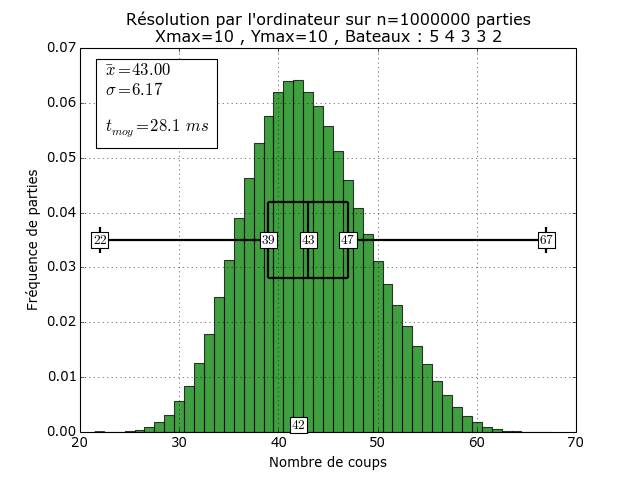
\includegraphics[scale=0.7]{./media/distrib_1000000.png}}
\end{center}

Notons les excellentes performances avec une moyenne de 42,06 coups par partie pour un temps moyen de seulement 31,2 ms.

La forme de cette distribution semble correspondre à une loi normale asymétrique.

%\chapter{Affichage console}
\chapter{Affichage console}
Le module \texttt{bn\_console.py} implémente l'interface en mode console.

L'idée de cette interface est de rendre hommage au style de jeu des années 80 en essayant d'en garder au maximum l'esprit.

\section{Préliminaires}
\subsection{Constantes graphiques}
Pour afficher les grilles nous utilisons des caractères graphiques en unicode (famille Box Drawing de codes U2500 à U257F). Ceux-ci donnent tous les outils afin de fabriquer des grilles, y compris avec des caractères gras. Pour des raisons de commodité, le code de chacun des caractères utilisés est stocké dans une constante (par exemple \texttt{CAR\_CX=u'\textbackslash u253C'} correspond à la croix centrale \texttt{┼}). La liste complète des codes des caractères utilisés est donnée en annexe \ref{annexe_codescar} page \pageref{annexe_codescar}.

\subsection{Effacer le terminal}
Le module \texttt{os} permet d'une part d'accéder à la version du système d'exploitation avec \texttt{os.name} et, d'autre part, de lancer des commandes système avec \texttt{os.system(commande)}. La combinaison de ces deux commandes permet facilement de pouvoir effacer l'écran en utilisant la commande \texttt{cls} sous Windows et \texttt{clear} sous Linux.

\subsection{Fusion des deux grilles}
Lors d'une partie contre un adversaire, il faut pouvoir afficher côte à côte la grille de suivi du joueur ainsi que sa propre grille avec, au fur et à mesure, les coups joués par l'adversaire. Afin de réaliser cette opération nous utilisons la fonction \texttt{fusion(chaine1, chaine2)}. Celle-ci prend en entrée deux chaînes de caractères et retourne la chaîne fusionnée de la façon suivante : chaque chaîne est convertie en liste en prenant comme séparateur le caractère de retour de ligne \texttt{'\textbackslash n'} grâce à la méthode \texttt{String.split('\textbackslash n')}. Ensuite, en prenant à tour de rôle les éléments de chacune des listes et en insérant un caractère de trait vertical entre les deux on crée la chaîne fusionnée. 

Le résultat peut être vu plus bas en page \pageref{deux_joueurs}.

\subsection{Autres fonctions d'affichage}
La fonction \texttt{centre(chaine, longueur)} centre la chaîne sur un espace de longueur donnée en insérant le nombre d'espaces nécessaires. Cette fonction sera utilisée pour l'affichage des noms des joueurs.

La fonction \texttt{boite(texte, prefixe, longueur)} permet d'encadrer le texte dans une boîte de longueur donnée, chaque ligne étant précédée d'un préfixe. Cette fonction sera utilisée pour afficher la liste des messages pour chaque joueur à chaque tour, les préfixe servant à identifier l'auteur du message.

Notons enfin qu'afin de pouvoir réutiliser le code de ce module dans d'autres contextes (comme une interface en \texttt{tkinter}), la fonction \texttt{print(*args)} a été encapsulée dans une fonction \texttt{info(*args)} de sorte qu'il suffit de surcharger cette dernière pour envoyer l'affichage ailleurs (par exemple dans une boîte de texte dans une fenêtre graphique)

\section{Affichage des grilles}
La classe \texttt{GrilleC(Grille)} hérite de la classe \texttt{Grille} en ajoutant uniquement les fonctions d'affichage.

\subsection{Affichage simple de la grille}
La méthode \texttt{GrilleC.make\_chaine(self)} crée la chaîne de caractères de la grille simple. En plus des coins, chaque case utilise 3 caractère horizontaux (ce qui permet de centrer un symbole) et 1 caractère vertical.

Pour cet affichage, on crée les lignes les unes après les autres (dans deux boucles impbriquées) en marquant les cases suivant les valeurs de \texttt{Grille.etat}. La seule subtilité provient des deux premières et de la dernière ligne (à cause des coins).


\subsection{Affichage de la grille avec ses propres bateaux en gras}
Cette partie est beaucoup plus délicate. L'idée est d'afficher une grille en entourant ses propres bateaux et en marquant les coups joués par l'adversaire (sa grille de suivi). C'est le rôle de la fonction \texttt{GrilleC.make\_chaine\_adverse(self, grille)}, où \texttt{grille} est soit sa propre grille de jeu, soit celle de l'adversaire si on veut tricher (pour les tests bien sûr...) ou en fin de partie, si on a perdu, pour avoir la solution. Par convention, comme \texttt{grille} est une grille de jeu, nous allons noter dans les explications les seuls états possibles par $1$ si la case est occupée par un bateau et $0$ sinon (ou si la case est hors grille).

Les contraintes que nous nous fixons sont les suivantes :
\begin{itemize}
\item Les bords des bateaux doivent être en gras
\item Les séparations à l'intérieur d'un bateau doivent être en clair
\item Lorsque deux bateaux se touchent par un coin, il faut bien sûr que ces coins soit en gras (soit une croix en gras)
\end{itemize}


Le bord de chaque case de la grille se fera sur la ligne du bas, la séparation verticale de gauche et le coin en bas à gauche. Le cas de la ligne horizontal juste sous les lettre sera fait à part, ainsi que la dernière ligne horizontale et la dernière ligne verticale de la grille (à cause du bord).

\begin{enumerate}
\item Première ligne, sous les lettres des colonnes : pour chaque case de la ligne $0$ on va tester son état, ainsi que l'état de la case de gauche (pour savoir si on est en début ou en fin de bateau, ou au milieu d'un bateau). On obtient les configurations suivantes (la case testée est celle de droite) :

\begin{verbatim}
   ┼───     ┿━━━     ╅───     ╆━━━
 0   0    1   1    1   0    0   1
\end{verbatim}


\item Lignes suivantes, jusqu'à l'avant dernière : ici c'est plus délicat car il faut tester, en plus de celle de gauche (pour la séparation verticale), la case en-dessous (pour la séparation horizontale) et celle en-dessous à gauche (pour le coin) pour obtenir les configuration suivantes (la case testée est celle en haut à droite) :

\begin{verbatim}
 1 │ 1    0 ┃ 1    0 ┃ 1    0 ┃ 1
   ┿━━━     ╄━━━     ╋━━━     ╂───
 0   0    0   0    1   0    0   1
  
 
 1 ┃ 0    1 ┃ 0    1 ┃ 0    0 │ 0    0 │ 0    0 │ 0    0 │ 0
   ╃───     ╂───     ╋━━━     ┿━━━     ┼───     ╅───     ╆━━━
 0   0    1   0    0   1    1   1    0   0    1   0    0   1
\end{verbatim}

\item Enfin, pour la dernière colonne va juste tester la case en-dessous, et pour la dernière ligne, on va juste tester celle de gauche. Pour la case tout en bas à droite il faudra juste finir en mettant un coin.

\begin{verbatim}
 0 │      0 │      1 ┃      1 ┃  
   ┤        ┪        ┨        ┩
 0        1        1        0
 
 1   1    1 ┃ 0    0   1    0 │ 0
   ┷━━━     ┹───     ┺━━━     ┴───

 1 ┃      0 │
   ┛        ┘
\end{verbatim}
\end{enumerate}

Au final, cela permet de construire toute la grille, dans tous les cas de figure possibles. Le résultat est visible sur la grille de droite ci-dessous.




\newpage
\section{Modes de jeu}
Après un écran d'introduction et un menu sommaire, le programme propose 3 modes de jeu :
\begin{enumerate}
\item Jeu en solo sur une grille aléatoire.
\item Résolution d'une grille aléatoire par l'ordinateur, avec mise en évidence des bateaux qu'il doit trouver (voir annexe \ref{annexe_algo_action} page \pageref{annexe_algo_action})
\item Jeu contre l'ordinateur (suivant l'algorithme vu en page \pageref{alogo_jeu}).

L'affichage sera alors le suivant :

\label{deux_joueurs}{\scriptsize
\begin{boxedverbatim}
                  ╔══════╗                     ┃                     ╔═════╗                   
                  ║ Toto ║                     ┃                     ║ HAL ║                   
                  ╚══════╝                     ┃                     ╚═════╝                   
    ┌───┬───┬───┬───┬───┬───┬───┬───┬───┬───┐  ┃      ┌───┬───┬───┬───┬───┬───┬───┬───┬───┬───┐
    │ A │ B │ C │ D │ E │ F │ G │ H │ I │ J │  ┃      │ A │ B │ C │ D │ E │ F │ G │ H │ I │ J │
┌───┼───┼───┼───┼───┼───┼───┼───┼───┼───┼───┤  ┃  ┌───╆━━━┿━━━┿━━━┿━━━┿━━━╅───┼───┼───┼───┼───┤
│ 0 │   │   │   │   │   │   │   │   │   │   │  ┃  │ 0 ┃   │   │   │   │   ┃ ◯ │   │   │   │   │
├───┼───┼───┼───┼───┼───┼───┼───┼───┼───┼───┤  ┃  ├───╄━━━┿━━━┿━━━┿━━━┿━━━╃───┼───┼───┼───┼───┤
│ 1 │   │   │ ◯ │   │   │   │   │   │   │   │  ┃  │ 1 │   │   │   │   │ ◯ │   │   │   │   │   │
├───┼───┼───┼───┼───┼───┼───┼───┼───┼───┼───┤  ┃  ├───┼───┼───┼───┼───┼───┼───┼───┼───┼───┼───┤
│ 2 │   │   │ ✖ │   │   │   │   │   │   │   │  ┃  │ 2 │   │   │   │ ◯ │   │   │ ◯ │   │ ◯ │   │
├───┼───┼───┼───┼───┼───┼───┼───┼───┼───┼───┤  ┃  ├───┼───┼───┼───┼───┼───┼───╆━━━╅───┼───┼───┤
│ 3 │   │   │ ✖ │   │   │   │   │   │   │ ✖ │  ┃  │ 3 │   │   │ ◯ │   │   │   ┃ ✖ ┃   │   │   │
├───┼───┼───┼───┼───┼───┼───┼───┼───┼───┼───┤  ┃  ├───┼───┼───┼───┼───┼───┼───╂───╂───┼───┼───┤
│ 4 │ ◯ │   │ ✖ │   │   │   │   │   │   │   │  ┃  │ 4 │   │   │   │   │   │   ┃ ✖ ┃   │   │   │
├───┼───┼───┼───┼───┼───┼───┼───┼───┼───┼───┤  ┃  ├───┼───┼───┼───┼───┼───┼───╂───╂───┼───┼───┤
│ 5 │   │   │ ◯ │   │   │ ◯ │   │   │   │   │  ┃  │ 5 │   │   │   │   │   │   ┃ ✖ ┃   │   │ ◯ │
├───┼───┼───┼───┼───┼───┼───┼───┼───┼───┼───┤  ┃  ├───┼───╆━━━┿━━━┿━━━┿━━━╅───╄━━━╃───┼───┼───┤
│ 6 │   │   │   │   │   │   │   │   │   │   │  ┃  │ 6 │   ┃   │   │   │   ┃   │   │ ◯ │   │   │
├───┼───┼───┼───┼───┼───┼───┼───┼───┼───┼───┤  ┃  ├───┼───╄━━━┿━━━┿━━━┿━━━╃───┼───┼───┼───┼───┤
│ 7 │   │   │   │ ◯ │   │ ◯ │   │   │   │   │  ┃  │ 7 │   │   │   │   │   │   │   │   │ ◯ │   │
├───┼───┼───┼───┼───┼───┼───┼───┼───┼───┼───┤  ┃  ├───╆━━━┿━━━╅───┼───┼───╆━━━┿━━━┿━━━╅───┼───┤
│ 8 │ ◯ │   │   │   │   │   │   │   │   │   │  ┃  │ 8 ┃   │   ┃   │   │   ┃   │   │   ┃   │   │
├───┼───┼───┼───┼───┼───┼───┼───┼───┼───┼───┤  ┃  ├───╄━━━┿━━━╃───┼───┼───╄━━━┿━━━┿━━━╃───┼───┤
│ 9 │   │   │   │   │   │   │   │   │   │   │  ┃  │ 9 │   │   │   │   │   │   │   │   │   │   │
└───┴───┴───┴───┴───┴───┴───┴───┴───┴───┴───┘  ┃  └───┴───┴───┴───┴───┴───┴───┴───┴───┴───┴───┘

<Toto> Coup (Entrée pour un coup aléatoire) : 
\end{boxedverbatim}
}
\normalsize

\end{enumerate}


Notons que chaque fois qu'une case est demandée au joueur, le programme teste la validité de sa réponse (chaîne qui n'est pas une case, case hors grille ou encore une case déjà jouée).

%\chapter{Interface graphique}
\chapter{Interface graphique}

Une interface réalisée grâce à la bibliothèque \texttt{tkinter} est codée dans le fichier \texttt{bn\_tkinter}. Dans cette interface, on a la possibilité de jouer seul sur une grille aléatoire, de voir l'algorithme de résolution (avec choix du niveau) et de jouer contre l'algorithme (avec choix du niveau de ce dernier et placement de nos bateaux).

Cette interface devait être réalisée par mon binôme, mais ce dernier ayant abandonné la formation quelques semaines avant la date de rendu de projet, j'ai dû la coder très rapidement. Je ne suis d'ailleurs pas totalement satisfait du résultat, même si elle est fonctionnelle (j'avais encore plein d'idées). C'est également pourquoi cette partie du rapport est moins détaillée, par faute de temps.

%\section{Principes de l'interface}
%
%Le point principal se situe dans la classe \texttt{GrilleTK(Grille)} qui implémente les fonctionnalités graphiques (avec un \texttt{canvas}) des grilles.
%
%%\medskip
%%
%%La fenêtre principale est basée sur une \texttt{Frame},  \texttt{main\_frame}, dans laquelle on va placer les grilles, ainsi qu'une fenêtre de texte. Entre chaque partie on l'efface en supprimant tous ses widgets enfants, obtenus dans la liste \texttt{main\_frame.pack\_slaves()}, grâce à leurs méthodes \texttt{destroy()}. 
%
%\medskip
%
%J'ai également créé deux fenêtres annexes pour placer nos bateaux (\texttt{PlaceWin}) et choisir pour le niveau de l'algorithme (\texttt{LevelWin}).
%
%\medskip
%
%Enfin les classes \texttt{JoueurTK(Joueur)} et \texttt{OrdiTK(Ordi, JoueurTK)} implémentent les fonctions graphiques, et notamment la gestion des événements souris, des joueurs.
%% Notons que pour pouvoir accéder à la boîte de texte \texttt{info} de l'interface principale qui affiche les informations de partie, on met l'attribut \texttt{name="info"} à ce widget et on y accède depuis la classe \texttt{JoueurTK(Joueur)} via \texttt{self.parent.children["info"]}, où \texttt{self.parent} est la frame principale (\texttt{main\_frame}).

\section{Affichage et gestion des grilles}
La classe \texttt{GrilleTK}, héritée de la classe \texttt{Grille} implémente le \texttt{canvas} sur sur lequel on va dessiner les grilles.

Sur ce \texttt{canvas}, on définit les marges \texttt{marge\_left} et \texttt{marge\_top} à gauche et en haut pour les intitulés des lignes et des colonnes, ainsi que la largeur des cases \texttt{largeur\_case}. 

\medskip

Les passages de coordonnées graphiques aux coordonnées des cases, et réciproquement, sont gérés via  une transformation affine par les méthodes \texttt{GrilleTK.coord2case(self, x, y)} et \texttt{GrilleTK.case2coord(self, case)}. Notons les méthodes \texttt{canvasx} et \texttt{canvasy} de l'objet \texttt{canvas} qui permettent de récupérer les coordonnées graphiques du curseur dans un repère associé au \texttt{canvas}.

\medskip

Enfin toute une série de méthodes vont permettre de marquer les cases suivant leur état, de colorier les bateaux adverses ou les bateaux coulés.  

\section{Fenêtre principale}
La fenêtre principale est constituée d'un menu pour lancer une partie et d'une \texttt{Frame} principale, \texttt{main\_frame}. Sur cette \texttt{Frame}, on va dessiner les grilles et une fenêtre de texte pour les informations de partie.

\medskip

Entre chaque partie on va effacer le contenu de cette \texttt{Frame} en supprimant tous ses widgets enfants (en fait ceux "packés") , obtenus dans la liste \texttt{main\_frame.pack\_slaves()}, grâce à leurs méthodes \texttt{destroy()}. 

\section{Gestion des joueurs et de l'ordinateur}
La classe \texttt{JoueurTK(Joueur)} fournit les interactions entre la grille du joueur et les événements souris. Afin de distinguer un joueur humain (qui peut donc agir avec la souris sur la grille), on a un attribut \texttt{Joueur.playable}.

Le fait de déplacer le curseur sur la grille de suivi met la case survolée en surbrillance et le fait de cliquer joue un coup.

Il faut également pouvoir afficher les informations sur la boîte de texte de la \texttt{Frame} parent. Ceci est possible  en mettant l'option \texttt{name="info"} à la boîte de texte \texttt{infos} de la \texttt{main\_frame} et en y accédant via \texttt{Joueur.parent.children["info"]}.

Enfin le placement des bateaux est implémenté comme détaillé ci-dessous.

\medskip

L'ordinateur, quant à lui, est géré par la classe \texttt{OrdiTK(Ordi, JoueurTK)} avec un paramètre \texttt{playable=False}.

\section{Fenêtres supplémentaire}
\subsection{Choix du niveau de l'algorithme}
La choix du niveau de l'algorithme s'effectue dans une fenêtre de type \texttt{Toplevel} dans la classe \texttt{LevelWin}.

Le niveau est déterminé dans un \texttt{Combobox} du sous-module \texttt{ttk} et, à chaque changement de valeur, un événement est déclenché pour, d'une part mettre à jour la description du niveau et, d'autre part, afficher une boîte de texte permettant de rentrer des paramètres supplémentaires pour les niveaux 4 et 6.

\subsection{Placement des bateaux}
Le placement des bateaux s'effectue dans une fenêtre de type \texttt{Toplevel} dans la classe \texttt{PlaceWin}.\\
Pour chaque bateau à placer, le principe est le suivant :
\begin{itemize}
\item Lorsque l'utilisateur clique une première fois sur la grille, sa case est mémorisée et le drapeau \texttt{first\_clic} est mis à \texttt{False}.\\
On détermine alors tous les bateaux valides démarrant sur cette case et on colorie leurs cases de fin.
\item  Lors du déplacement du curseur sur une case de fin possible, un aperçu du bateau est mis en couleur.
\item Lors du clic sur la case de fin, le bateau est validé et le drapeau \texttt{first\_clic} est remis à \texttt{True}.
\end{itemize}
Si on ferme prématurément cette fenêtre, les bateaux sont placés aléatoirement.

\medskip

On pourrait facilement améliorer cette phase (comme par exemple pouvoir faire glisser le bateau et changer son sens avec le clic droit, ou encore avoir un possibilité d'annuler son choix) mais le temps m'a manqué.


%\chapter{Guide des modules utilisés}
\chapter{Guide des modules utilisés}

%\chapter{Point de vue pédagogique}
\chapter{Point de vue pédagogique}

Bien évidemment, ce projet dépasse largement ce qui est exigible d'un élève (même très bon) de lycée. Certains points peuvent néanmoins être abordés en simplifiant certaines parties et en l'abordant soit comme une série de TP guidés (les élèves doivent coder le contenu des fonctions dont on leur donne le prototype), soit comme projet de fin d'année.
\begin{itemize}
\item La structure de la grille : un bon exemple de codage d'une structure complexe (définir les états des cases, utilisation d'un dictionnaire ou d'un liste double, tests des cases valides,...)
\item Le placement de bateaux : sûrement la partie la moins évidente, mais oblige à réfléchir sur la façon de définir un bateau 
\item L'affichage (simple) de la grille : utilisation de boucles imbriquées et de tests pour afficher les bons symboles, et gestion de la mises en page
\item Éventuellement une interface graphique en utilisant des boutons pour les cases
\item La possibilité pour un joueur de tirer sur une case
\item Une résolution de la grille par l'ordinateur avec uniquement des tirs aléatoires sur les cases vides
\end{itemize}



%\chapter{Conclusion}
\chapter{Conclusion}
%\section{Conclusion de Frédéric Muller}
Ce travail a été très stimulant et m'a pris de nombreuses heures (environ 200), mais j'y ai pris beaucoup de plaisir. Il a fallu mettre en place des structures de données pour avoir un projet minimal, l'algorithme de résolution et son optimisation, la mise en place des outils statistiques, et la construction de l'interface console ainsi que l'interface web.

Certes il reste des points à développer, comme la mise en place d'une architecture de jeu en réseau, ou une interface en \texttt{tkinter} qui devait être réalisée par mon binôme, mais je pense que ce projet est déjà bien abouti. 

La rédaction du rapport en \LaTeX\ a également été très plaisante, avec quelques figures réalisées avec tikz, l'affichage des caractères unicodes, ou encore la rapatriement automatique des docstrings (et des nombreux autres problèmes techniques qui m'ont permis de progresser). Cela m'a rappelé mes années d'étude, et notamment mon DESS IM dans lequel je faisais beaucoup de projets informatiques de ce type.

Enfin j'ai trouvé un grand intérêt dans l'obligation de rendre un travail propre et fini, ce qui n'est pas le cas dans un projet personnel, dans lequel on est moins exigeant. Cela faisait longtemps que je n'avais pas fait ça et, rien que pour ça, je suis heureux d'avoir suivi cette formation.


\end{document}